\documentclass[UTF-8]{ctexart}


\usepackage{url}
\usepackage{cite}
\usepackage[version=4]{mhchem}
\usepackage{graphicx}
\usepackage{subfigure}
\usepackage[a4paper,top=2cm,bottom=2cm,right=3cm,left=3cm,marginparwidth=1.75cm]{geometry}
\usepackage{amsmath}
\usepackage{upgreek}

\title{人机交互中的电磁学原理}
\author{闫皓铭 \\ 元培学院 2300017744}
\date{Autumn, 2024}


\begin{document}
\maketitle

\section{引言}
作为整合科学专业的学生,我一直试图在与生物学相关的多学科交叉的领域中,寻找一些和电磁学课程联系紧密的,有趣新颖的话题和对象,作为本次读书报告的主题。
最终决定阅读和“人机交互”相关的书籍,并把我的一些收获总结在这篇报告中。

人机交互在我们的日常生活中已经非常普遍了,这里所谓的“机”,以手机、平板等电子设备为典型代表。
而电子设备中,自然涉及到诸多电磁学知识作为其原理,与此同时,在不同应用场景中,展现出很大的灵活性、多样性与实用性。
而人机交互也离不开人的感官和感觉。交互方式通常涉及“视觉”“听觉”和“触觉”。
为了实现更好的人机交互效果,相关电子设备的设计都基于人类的生物学特征和基本的生物学原理。

通过相关资料与书目的阅读,我对很多日常中习以为常的设备的工作原理有了更深刻的认识,
对电磁学理论的应用有了更丰富的认识,对生物学相关知识有了更生动的认识。
\section{涉及视觉的交互——屏幕} 
\subsection{屏幕显示技术:侧重墨水屏显示机理}
\begin{figure}
    \centering
    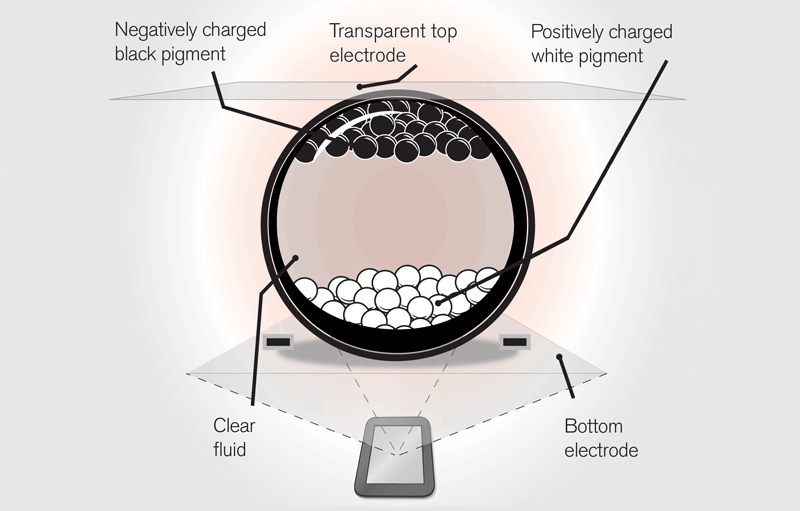
\includegraphics[width=0.4\linewidth]{../Figures/epaper-single ball.png}
    \caption{“双颗粒模式”,类似点电荷\cite{ePaper-web}}
    \label{双颗粒}
\end{figure}
\begin{figure}
    \centering
    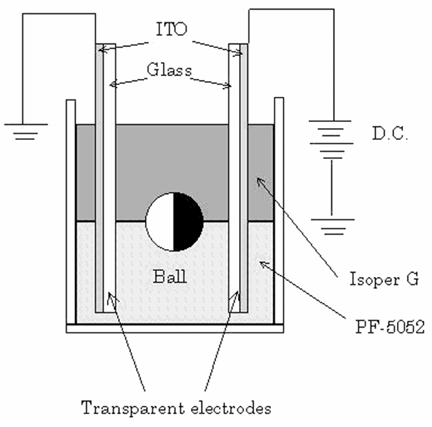
\includegraphics[width=0.4\linewidth]{../Figures/epaper-dipole.png}
    \caption{“单颗粒模式”,类似电偶极子\cite{ball}}
    \label{单颗粒}
\end{figure}
电子显示器件分为主动发光与非主动发光两种类型,墨水屏属于非主动发光的那一类,即,需要借助外界光源进行显示的技术\cite{tablet}。
上学期,为了方便整理笔记,我买了华为的MatePad Paper这款产品,其中就运用了墨水屏(ePaper)的技术。
有趣的是,这种显示技术与常见的液晶显示(LCD)和有机发光二极管(OLED)的发光机理尤其是显示效果有明显不同。
其独特优势和显著性的缺陷并存,使得它在市场中始终顽强地占有很小的一席地。
因而我想了解一下墨水屏(ePaper)的工作机制,进而理解它的功能特性,以及应用场景。

\subsubsection{工作机制的概览}
我所关注的墨水屏,属于粒子移动型ePaper技术\cite{tablet},原理是所谓“电泳”。
这种“电泳”的原理和我们在生化实验中使用的DNA凝胶电泳和蛋白质SDS-PAGE电泳有类似之处,都是利用了分散系中微粒子在电场中的移动。
当然,粒子是带电荷的。

但是电泳显示器分为“单颗粒模式”与“双颗粒模式”。从电磁学角度来看,“双颗粒模式”中的每一个颗粒可以抽象成\textbf{点电荷},而“单颗粒模式”中的单颗粒,可以抽象成\textbf{电偶极子},参考图\ref{单颗粒}和图\ref{双颗粒}。

墨水屏的显示机理的一个最显著光电特性是它的“双稳态”特性,见图\ref{双稳态}。
\begin{figure}
    \centering
    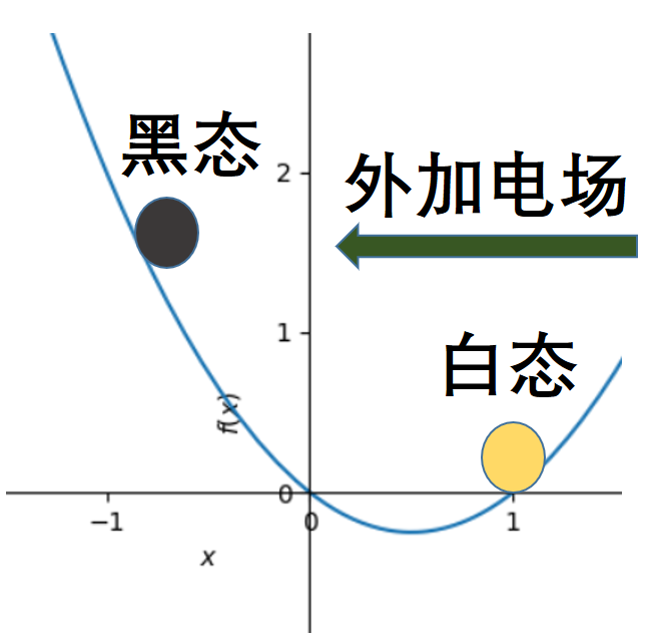
\includegraphics[width=0.4\linewidth]{../Figures/monostable.png}
    \caption{单稳态光电特性}
    \label{单稳态}
\end{figure}
\begin{figure}
    \centering
    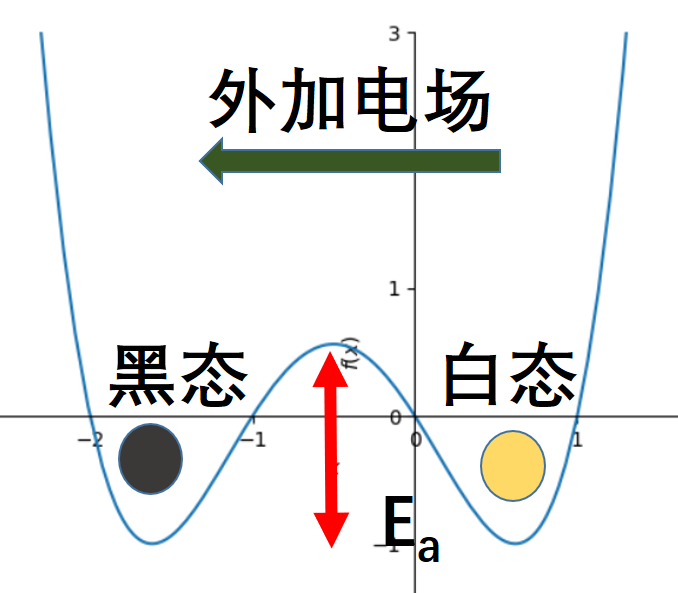
\includegraphics[width=0.6\linewidth]{../Figures/bistable.png}
    \caption{双稳态光电特性}
    \label{双稳态}
\end{figure}
双稳态光电效应的好处在于,它能够使影像在没有外加驱动电压的情况下,依旧保持稳定,拥有记忆效应。
只有影像进行切换的时候,才需要电源,因而更加节省电能。
而单稳态下的光电特性,如图\ref{单稳态}所示,需要外加电压/电场来维持显示画面,不具备这一特点。
我使用的MatePad Paper在锁屏乃至关机的状况下,都会显示一副灯塔的画面。我想,这一定是利用了双稳态的光电特性。
我想,这也是在产品设计过程中,巧妙地利用物理原理,不仅节省了能量,还给用户创造了更好的体验效果。


衡量电泳显示器件的一个重要参数是电泳迁移率($\mu$)。从定义上看,这和老师补充的“载流子迁移率”是一致的。
$$
\vec{v}=\mu \cdot \vec{E}
$$
但是,这里电泳微粒的尺寸,应该比电子大很多。

\subsubsection{双稳态的成因与影响}
首先,如前所述,双稳态的光电特性,使得显示器更加节省能量,只在切换页面的时候需要能量供给,维持画面不需要能量。
但矛盾总有两个方面,这也带来了页面切换速率的低下,显示的开关时间达到几十毫秒\cite{tablet},用户可以感受到刷新的过程。
这样低下的刷新速率是不支持播放视频的,因为每秒能进行的刷新次数要低于视频每秒的帧数。

具体而言,对于这样的双稳态特性,可以类比一元的化学基元反应理解。
活化能的大小,决定了单侧反应的速率常数。
弛豫时间(状态切换等待时间的期望值)是速率常数的倒数。
$$
k(T)=Ae^{-\frac{E_a}{k_BT}}
$$
$$
<t>=\frac{1}{k}=\frac{e^{\frac{E_a}{k_BT}}}{A}
$$
(t作为随机变量,满足指数分布$P(t)=ke^{-kt}$,其期望值为$<t>=E(t)=\frac{1}{k}$)


从中可见,更高的能垒会带来更长的弛豫时间,从而降低了刷新速率。
可是为什么会出现这种双稳态的光电特性呢?
总的来看,是因为影像切换的过程,微观上粒子从一个稳态出发,到达另一个稳态。

对于“单颗粒模式”(旋转双色球)而言,油性介质的密度与双色球接近,
当电场撤出后,已经旋转到位的小球便保持之前的旋转排列方式,宏观上就将显示内容保存下来了\cite{tablet}。

对于“双颗粒模式”而言,每一个像素的电路运用了TFT(Thin Film Transistor),和储存电容。
在电容放电,外电场驱动离子迁移,粒子迁移形成退极化场这一系列过程后,最终的效果也是体系具备两个稳态。
这一点我尚需要进一步了解。
\subsubsection{进一步讨论}
这学期,我在使用MatePad Paper阅读细胞生物学教材的时候很快便意识到该产品的一个很大缺陷,即,无法进行彩色显示。
从前面关于显示机制的讨论中,我们可以看到黑白球在技术上比彩色球更容易实现,更容易控制。
然而近期也出现了一些可以彩色显示的墨水屏,有的涉及到各种滤光片,有的将一个球的不同方位涂上不同颜色...\dots
这一技术需要攻克的难题还有很多,但是它的特性与优势也是明显而与众不同的。

除此之外,在这样一个与应用联系紧密的商业领域,技术的进步与市场的规律共同决定了事物的发展。
早期企业形成的先发优势,以及市场整体呈现的波动规律比如“液晶周期”,都对显示技术产生着深远影响。
\subsection{屏幕触控技术}
我主要调查了解了三种触控技术:电阻式、电容式、压电式。
它们的技术原理各不相同,具备的功能与应用场景也有很大差别。
然而就电磁学原理的角度来看,它们主要运用了静电场和电介质的知识。
\subsubsection{电阻式触控:联系静电场与直流电路部分知识}


电阻式触控的基本原理是基于匀强电场,电势与位移成正比:
$$
E = -\nabla \varphi=\text{定值}   
$$
$$
\frac{\text{测量电势}}{\text{供电电压}}=\frac{\varphi_1}{\varphi_2-\varphi_1}=\frac{d_1}{d_2-d_1}=\frac{\text{测量位置}}{\text{屏幕宽度}}
$$
匀强电场是在上下两层电阻中形成的\cite{Touch},参考图\ref{电阻式触控原理}。
上下两侧电场相互正交,是为了测量$(x,y)$两个坐标。
上下两层的电场是交替形成的。工作机制是这样的:上层形成电场,下层进行测量;下层形成电场,上层进行测量;二者交替进行。
\begin{figure}
    \centering
    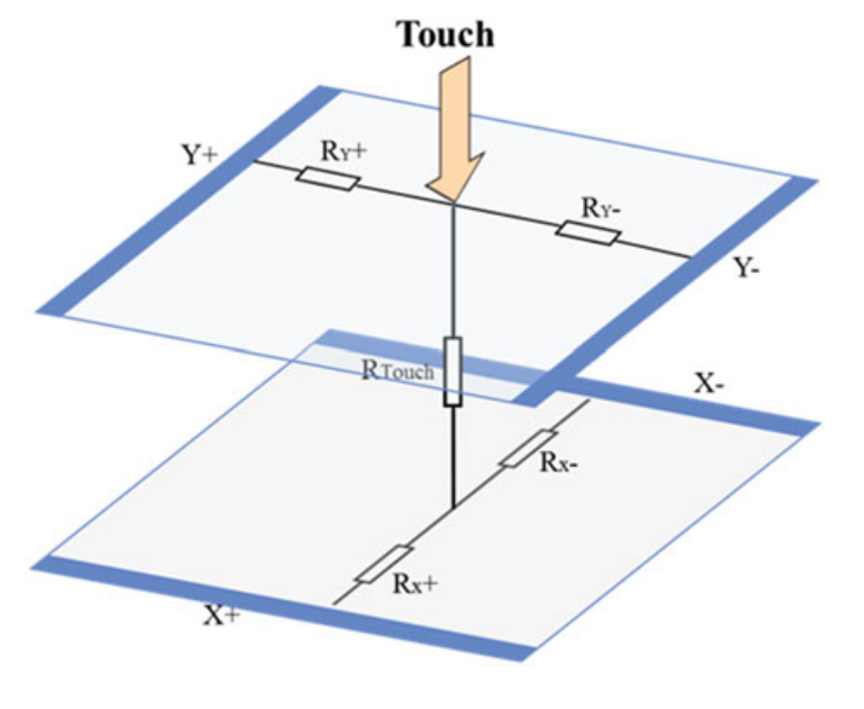
\includegraphics[width=0.5\linewidth]{../Figures/resistive.png}
    \caption{电阻式触控原理\cite{Touch}}
    \label{电阻式触控原理}
\end{figure}
从材料的角度看,上下两层导电层是\ce{In}与\ce{Sn}的氧化物,叫做(Indium Tin Oxide, ITO),具有透明的良好属性\cite{ITO}。
导电层之间用绝缘材料隔开,只有在用力按压触摸时,才相互接触,从而可以互相测量电势,进而探测位置。

这种电阻式的触控对于施力物体的电学性质没有要求。
这既是优点,也是缺点。
根据我的观察,咱们学校文史楼一些教室安装的屏幕就具有这种特点。
用塑料的签字笔,便可以实现对屏幕的触控,从而可以在屏幕上写字。
从而可以推断,该屏幕大概率是电阻式的触控屏。
但我们的手机显然不是这样的,因为从这个原理来看,电阻式的触控屏只能支持单点触控,不能实现多点触控。
此外,这会增加手机误触的风险。比如揣在兜里的手机可能会被意外触控。

\subsubsection{电容式触控:联系电容器部分知识}

\begin{figure}
    \centering
    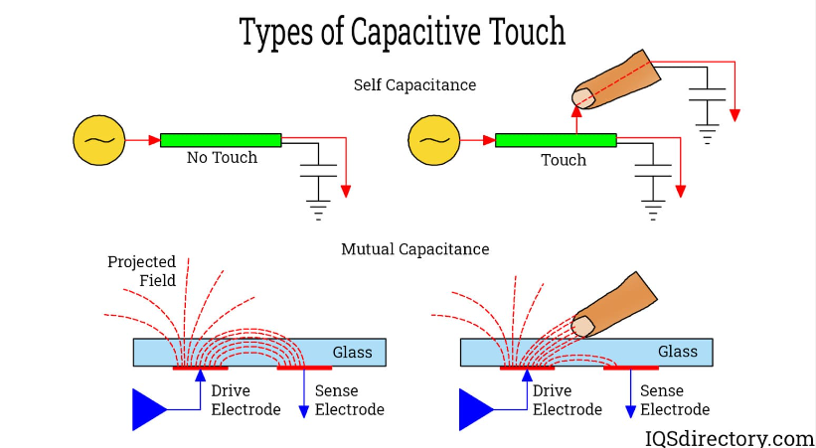
\includegraphics[width=0.7\linewidth]{../Figures/capacitive.png}
    \caption{电容式触控原理\cite{Capacitive}}
    \label{电容式触控原理}
\end{figure}

电容式触控种类繁多,我在这里分析两类。一类是所谓“自电容”类型,另一类是“互电容”类型。
它们的工作原理参考图\ref{电容式触控原理}。

首先可以明确的是,在这个模型中,人视作导体,并且接地。
手指与极板接近,则相当于增加了一个电容。
两种机制的最大区别在于,“自电容”测量的是驱动电极与大地之间的电容,而“互电容”测量的是驱动电极与接收电极之间的电容。

在“自电容”机制中,手指(此处视作导体)的接近,相当于给原本存在的寄生电容并联了一个电容。
从而总电容(待测电容)\textbf{增大}。

而在“互电容”中,驱动电极与接收电极之间形成的电容器是开放式的,这一点与常见电容器不同。
手指,作为导体的靠近,使得电场线更多地指向手指。
换言之,手指改变了原本的电场分布(这个电场被称为投射电场)。
从图\ref{电容式触控原理}可见,这相当于减少了有效正对面积,从而手指的靠近使被测电容值(驱动电极与接收电极之间,而非总电容)\text{减小}\cite{Capacitive}。

电容的测量涉及反复充放电的过程。而对于位置的确定,经过了对全平面多个测量子区域的反复扫描。
这种扫描的时延不为我们用户所感知,但无疑是工程师考虑的重点。
“互电容”因为机制复杂,所以扫描周期更长,时延更大。

一个有趣的现象是,“自电容”机制支持一点触控或两点放缩(可以双指放大或缩小页面),却也仅支持放缩操作。
“互电容”则可以支持更多点的触控。

“互电容”支持多点触控相对好理解,因为它将全平面划分为多个子区域,并且彼此独立(相邻两极板间的电容),测量互不干扰。

“自电容”则不然。由于它测量的是对地的总电容,从而各个子区域并不独立。
具体结构可以参考图\ref{“自电容”机制中的邻顶点与对顶点}中的示意。
具体来讲,各列与各列独立,但是一列之内不可区分。各行与各行独立,但是一行之内不可区分。
当仅有一个触摸点的时候,取一行与一列的交点即可唯一确定位置。
但是有两个触摸点的时候,两行两列形成四个交点,究竟是哪两个点?结果并不能唯一确定。
有趣的是,这并不影响双指放缩的操作,因为这个操作只关心双指之间的距离,与具体位置无关。
从而这一功能是可以实现的。
\begin{figure}
    \centering
    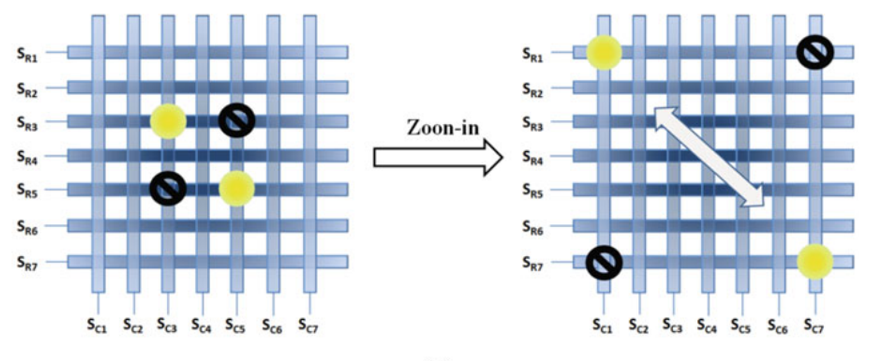
\includegraphics[width=0.9\linewidth]{../Figures/self.png}
    \caption{“自电容”机制中的邻顶点与对顶点不可分辨性与双指放缩操作的可行性\cite{Touch}}
    \label{“自电容”机制中的邻顶点与对顶点}
\end{figure}


电容式较电阻式有明显优势,更多地被精密的屏幕所采用。
但也应注意到,电容式触控只关心电学性质,而不能够探测施加的力的大小,而电阻式可以。
此外,这也解释了为什么我们冬天戴手套很难操作手机。因为手套的绝缘面料阻断了这一感应机制。
\subsubsection{压电式触控:联系电介质部分知识}
压电现象指的是,施加压力后电介质表面产生电荷。压电现象的逆效应也被实验证实。
也就是说,压电现象的正逆效应是电信号与力学信号转化的又一座桥梁(电磁感应或许是最经典的桥梁)。

与课内学习的电介质极化机制不同,压电效应的电介质极化来自于外界施加压力而非外电场。
这种神奇的现象,本质上源自于分子结构缺乏中心对称性,参考图\ref{压电效应的分子机制 }。
\begin{figure}
    \centering
    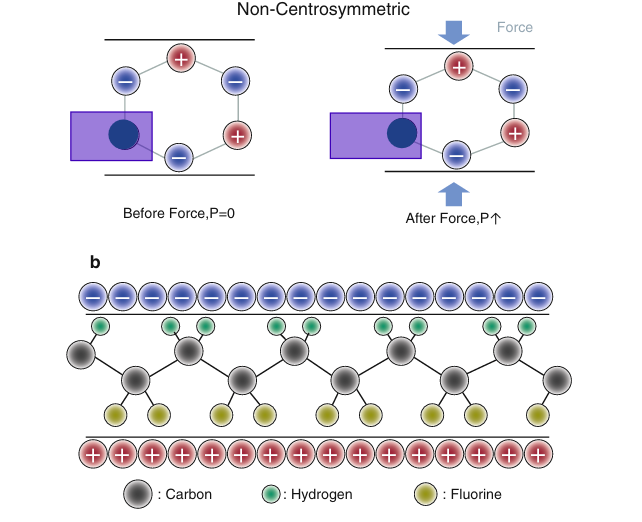
\includegraphics[width=0.7\linewidth]{../Figures/piezoelectric.png}
    \caption{压电效应的分子机制(poly(vinylidene fluoride), PVDF)\cite{Touch}}
    \label{压电效应的分子机制 }
\end{figure}
电极化强度矢量由应力决定:
$$
P=\tilde{d}\sigma\quad,\sigma\text{表示应力}
$$
电极化强度矢量决定了表面电荷密度:
$$
\sigma_{e}=\vec{P}\cdot \vec{n}
$$
电压由电荷产生:
$$
U=\frac{Q}{C}=\frac{\sigma_{e}S}{\frac{\varepsilon _0 \varepsilon _r S}{t}}=\frac{\tilde{d}\sigma S}{\frac{\varepsilon _0 \varepsilon _r S}{t}}=\frac{t\tilde{d} }{\varepsilon _0 \varepsilon _r}\cdot{\sigma}
$$
而归根结底,电压是由应力决定的。
\begin{figure}
    \centering
    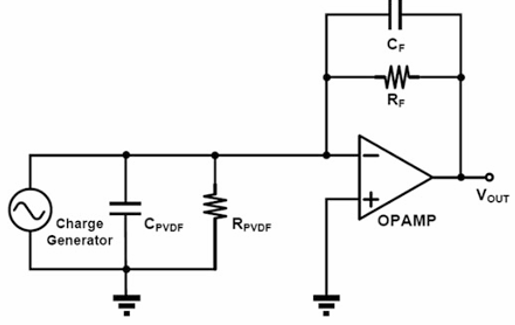
\includegraphics[width=0.6\linewidth]{../Figures/opamp.png}
    \caption{运算放大器构成的积分器实现电荷增益\cite{Touch}}
    \label{运放}
\end{figure}


而压电效应产生的电荷与电压都是很小的。实际应用中,采用了运算放大器进行信号增益。
具体来讲,使用了一个由运算放大器构成的电荷放大器\cite{circuit},实现对电荷的放大与测量,如图\ref{运放}。
为了达到更好的电荷增益效果,应该选用较小的电容器$C_F$。
$$
V_{out}=-\frac{Q}{C_F}
$$
上式中$Q$是$C_F$ 左极板所带电荷量,由于运算放大器的“虚短特性”,$C_{PVDF}$,$R_{PVDF}$两端与大地等势,电势为零,不积累电荷也不导通电流。
从而压电效应产生的电荷量全部集中在了$C_F$左极板。

而由于触控由生物体发出,是一个低频信号,所以应采用较大的电阻器$R_F$,与电容器一起构成一个低通滤波器。
$$
f_{\text{cut off}}=\frac{1}{2\pi R_FC_F}
$$

上面关于截止频率的分析,实际上我们在教材例题中处理过。电磁学教材,第284页例题7,计算过电阻与电容并联后的阻抗$Z$。
$$
Z=\frac{R_F}{\sqrt{(1+(\omega R_FC_F)^2}}
$$

从而可以定义特征频率$f_{\text{cut off}}$为阻抗衰减到$0.5R_F$时候的频率,参考图\ref{截止频率的定义}。
\begin{figure}
    \centering
    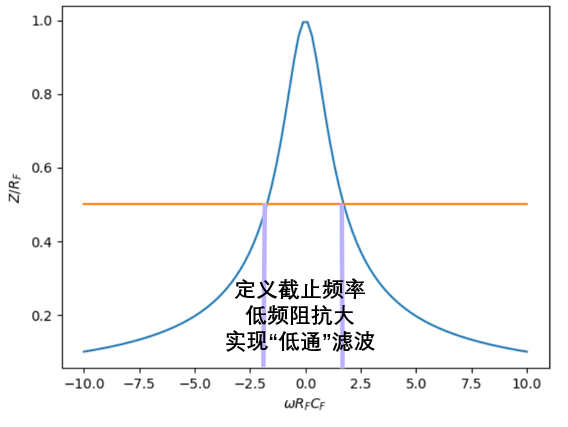
\includegraphics[width=0.6\linewidth]{../Figures/cut off frequency.png}
    \caption{截止频率的定义}
    \label{截止频率的定义}
\end{figure}

压电效应技术并不十分成熟,还在广泛的研究之中。
但是,它和电容式的触控联合使用,可以同时实现对力学量的测量,以及多点触控等良好的控制效果。
此外,由于压电效应本身并不依赖于供电电源,这使得它的功耗较低。
除了显示屏幕,这种新技术也被用于可穿戴电子设备,进一步丰富了人机交互的途径。


\section{涉及触觉的交互}
\subsection{触摸行为的生物学特质}
准确刻画触摸行为的生物学特质至关重要,比如在打电话的时候要排除掉面部和手机屏幕接触引发的误触干扰。
要准确的计算出触摸中心,而且计算方法应该对于成人和小孩都适用。
这个过程中,除了要关注手指的几何参数(长宽以及曲率)还要关注电学参数(电导),这一点对于电阻式触控没有影响,但对电容式触控影响显著。

此外,在书写、绘画等过程中,用力的大小通常转化为线条的粗细。
那么这就要求对人用力的相对值,有一个较为准确的测量方法。

与此同时,工程上还要考虑到噪音处理的问题。
鉴于人的触摸频率是比较低的,在10HZ一下,所以实际电路中,涉及许多低通滤波器来过滤噪音。
\subsection{触觉交互的必要性}

单纯的基于视觉与听觉的人机交互具有很大的局限性。
这需要我们使用者聚精会神于电子产品,并且在强光照条件下,视觉交互困难,在公共场合下,听觉交互会引起尴尬...\dots
而良好的触觉交互,同样可以起到很好的控制于感知的作用。
在前面有关触控屏幕的部分,我汇报了人如何通过触摸控制机器。
接下来,我将关注于,机器如何产生振动,进而通过触觉,向用户传递信息。
\subsection{振动的产生机制:联系电磁感应部分知识}
\begin{figure}
    \centering
    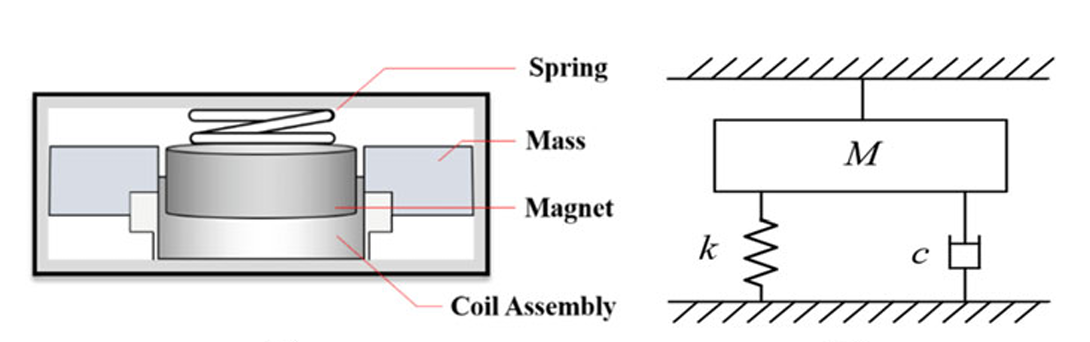
\includegraphics[width=0.6\linewidth]{../Figures/oscillator.png}
    \caption{线性共振激励发生器\cite{Touch}}
    \label{线性共振激励发生器}
\end{figure}
\begin{figure}
    \centering
    \subfigure[弹簧劲度系数的影响]{
        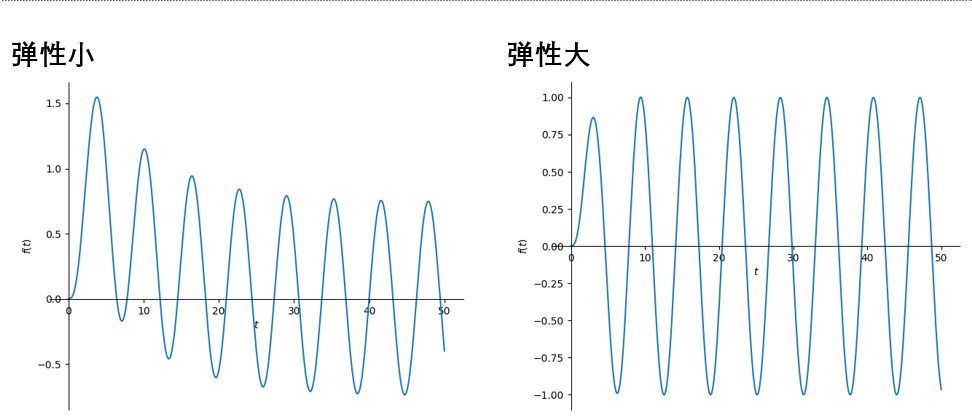
\includegraphics[width=0.5\linewidth]{../Figures/elastic.png}
    }
    \subfigure[电磁阻尼的影响]{
        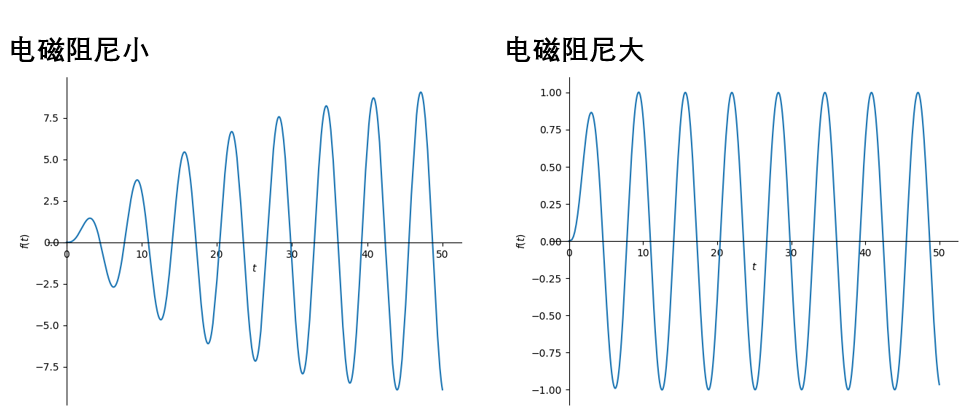
\includegraphics[width=0.5\linewidth]{../Figures/friction.png}
    }
    \subfigure[物块质量的影响]{
        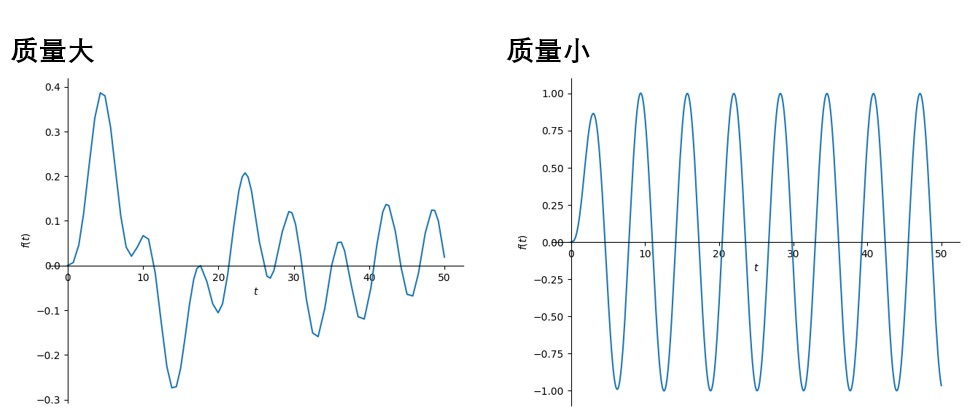
\includegraphics[width=0.5\linewidth]{../Figures/mass.png}
    }
    \caption{振动模式的三种影响因素}
    \label{振动模式}
\end{figure}

振动的产生显然离不开电动机。经典而传统的方法是通过直流电驱动一个电机,而负载是一个质量不均匀的物块,进而产生了振动。
在此基础上,“线性共振激励发生器”通过交流电驱动,结合了弹簧(力正比于位移),电磁阻尼(力正比于速度)和惯性力(力正比于加速度),在数学上构成了一个二阶线性常微分方程,交流信号为方程的非齐次项,参考图\ref{线性共振激励发生器}。
$$
M\frac{d^2}{dt^2}x+c\frac{d}{dt}x+kx=A\sin(\omega t)
$$

这相比于直流电机,更容易控制输出的振动模式,具有更快的响应速度。
为了从定性的角度,理解弹簧劲度系数,电磁阻尼系数和物块质量对振动模式的影响,我用计算机模拟了一下几种状况,加以对比。

从图\ref{振动模式}中可以看出,电磁阻尼大可以以更长的时间达到振幅更大的平衡态;
质量更大,会使得振动起始阶段不规则;弹性过小,起始阶段会呈现出整体性波动。

除此以外,振动还可以通过压电效应的逆效应产生。
这样的机制,需要更大的电压,却拥有更低的功耗。
\subsection{机械振动与交流电的类比分析}
根据电磁学教材第293页,图7-23(a)的RLC串联电路, 我们可以列以下微分方程:
$$
L\frac{d^2}{dt^2}q(t)+R\frac{d}{dt}q(t)+\frac{1}{C}q(t)=e(t)=B\sin(\omega t)
$$
将这样一个式子和机械(含阻尼)振动的微分方程对比:
$$
M\frac{d^2}{dt^2}x(t)+c\frac{d}{dt}x(t)+kx(t)=A\sin(\omega t)
$$
不难发现,这里有很强的类似性。从数学上来看只是一些简单的变量代换:
$$
M \sim L;\ R \sim c;\ k \sim x
$$
同时可以仿照交流电路定义的阻抗,定义机械阻抗\cite{newconcept}。
$$
Z_{\text{电}}=\frac{U}{I}\sim Z_{\text{机械}}=\frac{F}{v}
$$
这样,电磁学中,交流电部分关于串联谐振电路中谐振曲线的相关讨论均可以迁移至此。
其中谐振曲线的尖峰很好的解释了,振动产生器命名“线性共振激励发生器”,“共振”二字的含义。

反过来再从物理的角度,理解数学上的变量代换,不难发现,这一套类比关系(同构关系)是十分自然且符合直观的。
这样一套类比关系的基础是位移对应电荷、速度对应电流:
$$
x(t)\sim q(t);\ v(t)\sim i(t)
$$
质量阻碍物体速度改变,电感阻碍电路电流改变。这种改变分别需要外力的作用与外电压的作用:
$$
F=M\frac{d^2}{dt^2}x(t)\sim \ U=L\frac{d^2}{dt^2}q(t)
$$
惯性力与自感电动势对应,分别与外力和外电压平衡:
$$
F_{\text{惯}}\sim\ \mathcal{E} 
$$
粘滞阻力是一种耗散力,不具备之间反演不变性。电阻发生也是一种耗散作用,不具备时间反演不变性。二者都是不可逆的过程。
而且,对于阻力而言,阻力正比于速度;对于电阻而言,压降正比于电流:
$$
F_{\text{阻}}=c\frac{d}{dt}x(t)\sim \ U=R\frac{d}{dt}q(t)
$$
对于弹簧而言,形变积累会引起恢复力;对于电容而言,电荷量积累会产生电压:
$$
F_{\text{弹}}=kx(t)\sim\ U=\frac{1}{C}q(t)
$$

虽然上述二阶常微分方程所提供的类比关系就这么多,但我们可以顺着这一思路继续探索一些新的观点。

比如弹簧的形变从能量角度看,位移会产生弹性势能;电容器积累电荷,从能量角度看,电荷会产生静电能:
$$
E_p=\frac{1}{2}kx^2(t)\sim\ W_e=\frac{1}{2}\frac{1}{C}q^2(t)
$$
物体的运动(位置随时间改变)会产生动能;电路的电流(电荷随时间改变)会产生自感磁能:
$$
E_k=\frac{1}{2}mv^2(t)\sim \ W_{\text{自}}=\frac{1}{2}Li^2(t)
$$
从功率的角度看:
$$
P_{\text{机械}}=Fv(t)\sim \ P_{\text{电路}}=Ui(t)
$$
回到对微分方程的讨论上来,交流电部分建立的分析方法应该对于力学系统同样适用。
复数解法与向量法共同针对的都是“正弦稳态响应”\cite{circuit},而没有涉及暂态过程。

从处理微分方程的一般方法来看,Laplace变换、Green函数方法与时域经典解法等方法对二者也都同样奏效。
只不过在求解“正弦稳态响应”时都显得有些小题大做了。

\subsection{关于力学与电磁学类比的一点讨论}
从数学上看,“类比关系”实际上应该是“同构关系”。
能给人带来启发性的类比关系(展现出类似的物理规律),就像同构映射一样要“保持运算(算律)”。

从空间的角度出发(距离平方反比规律),会自然的构建物体质量与物体电荷的类比关系,引力场与静电场的类比关系,引力势与静电势的类比关系。
这一套类比关系(同构关系),从数学上看,主要是保持了对于空间上的微分积分运算律(梯度运算和曲线积分);从物理上看,主要是保持了有关“场”的物理规律。

从时间的角度出发(关于时间的常微分方程ODE),会自然的构建物体位移与电路元件电荷的类比关系,速度与电流、力与电压等的类比关系。
这一套类比关系(同构关系),从数学上看,主要是保持了对于时间上的微分积分运算律(对时间求导);从物理上看,主要是保持了“动力学”(运动)相关的物理规律。

力学与电磁学两个不同的体系,根据物理规律的不同侧重(空间与时间),可以建立两套不同的类比关系,并且带来一定的启发性。
我觉得这一点是有趣的,所以顺便也写在了读书报告之中。

\section{总结}
在本次有关人际互动中的电磁学原理的阅读中,我发现基础科学在应用领域中也会展现出蓬勃的活力。
不同的应用场景,给人以“乱花渐欲迷人眼”的感觉,但其中的电磁学原理是一贯的,展现了电磁学的基础性地位。
与此同时,我也意识到,工程上,要想产生有用的产品,还有很多技术挑战需要突破。
此外,和产业界、商业界的接触中,技术与市场共同决定了一个领域的发展。
基础研究、工程技术、转化科学、经济学等来自不同学科的知识与规律,共同决定了一个领域的发展。

另外一个角度讲,我觉得这个选题也让我对一些平日里已经熟视无睹的事物产生了更加深入的认识。
我们常用的手机以及电子产品的内部,涉及到的理论知识和技术原理是十分丰富的,集中体现着前人的智慧与劳动,值得细细品味。










\bibliographystyle{plain}
\bibliography{references}
\end{document}